\chapter{A Case Study: The RecipeWorld}\label{ch: case study}

The context of choice for this case study, which shows how the developed framework works, is the RecipeWorld, an \ac{ABM} model developed by \textcite{Fontana2015recipeWorld}.

In RecipeWorld,
\marginnote{the RecipeWorld}%
networks arise naturally from the interactions of autonomous agents, whereas each agent is engaged in a series of steps -- just like following a recipe -- towards a specific goal. It depicts a model wherein each agent operates independently, yet their actions contribute to creating a more extensive, interconnected network. This world is not pre-planned or engineered to form a network; instead, the network takes shape as a by-product of agents working through ordered sequences of tasks, much like individual workers assembling parts on a production line.

Each agent in RecipeWorld has a role, capabilities, and purpose, represented by \enquote{orders} that contain technical instructions or objectives. To achieve these objectives, agents execute \enquote{recipes,} which are sequences of steps. For example, a recipe agent might need to perform one action before another, or it might be required to complete several tasks simultaneously, similar to how ingredients are combined in specific ways when following a recipe in cooking or a sequence of steps in factory production. These steps, or events, activate agents, guiding their interactions with other agents and forming links between them. As recipe agents with their assigned tasks move from agent to agent, the network grows dynamically, mimicking the real-world flow of goods in production or information in communication.

Over time, the network emerges out of the repetitive yet purposeful actions of agents. These links can strengthen with each repeated interaction, highlighting frequently used connections, while weaker connections fade. As the network is established, it reflects the standard actions of its agents. 

\primjer{
    Consider a network of factories (i.e. \enquote{service providers}) where each unit specialises in a particular task within a production sequence -- we shall call this specialisation an offered \enquote{service}. Recipe agents (i.e. \enquote{service consumers}) move from one factory to another based on their respective recipes and their required services. This commotion enables connections to be formed based on the sequence of steps completed. 
}{Service providers and consumers}

RecipeWorld’s organic network creation has broader implications. It offers a neat way to test ideas in a simulated environment, observing how policies and other features might affect interconnected systems, from production lines to social services. Moreover, RecipeWorld’s networks can help reverse-engineer observed real-world networks, inferring the underlying behaviours from which they emerged. Rather than setting out to control or shape the network from above, RecipeWorld allows networks to emerge naturally from the ground up, showing how order, complexity, and efficiency can spontaneously develop from individual agents' simple, goal-oriented actions.



\section{The Ontology}

The example ontology comprises two particular types of agents: \mintedInline{Factory Agent} and \mintedInline{Recipe Agent}. These two subconcepts of the \mintedInline{Agent} concept reflect the service-consuming and service-providing agents of the RecipeWorld model described above. The three provided individuals per the above mentioned concept are enough to showcase how the agent individuals are translated to their respective implementation templates.

There are two \mintedInline{Plan} individuals in the example ontology.
\lookAt{\cref{fig: Example Produce part plan}}%
Each of those is related to a set of \mintedInline{Action}
\lookAt{\cref{fig: Example Communicate plan}}%
individuals that can be used to reach specified \mintedInline{Objective} individuals and are implemented using the connected \mintedInline{Behaviour} individuals. Furthermore, three \mintedInline{Role} individuals are defined, some of them providing specific \mintedInline{Behaviour} individuals. Individual \mintedInline{Agent} individuals
\lookAt{\cref{fig: Example agents and roles}}%
are connected to specific \mintedInline{Role} individuals. Lastly, there are several \mintedInline{Behaviour} individuals in the ontology, some of them modelled as \mintedInline{State} individuals related to \mintedInline{Finite State Machine Behaviour} individual.

\begin{figure*}
    \centering
    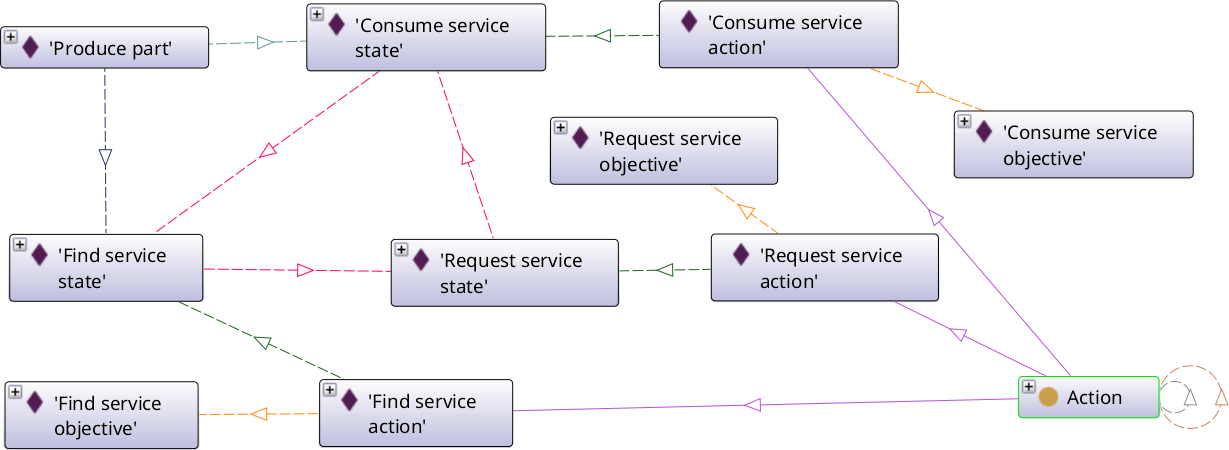
\includegraphics[width=\linewidth]{Deliverables/Phase 1/Figures/Example Produce part plan.png}
    \caption{Selected individuals related to the \mintedInline{Produce part} individual of concept \mintedInline{Plan}}
    \label{fig: Example Produce part plan}
\end{figure*}

\begin{figure}
    \centering
    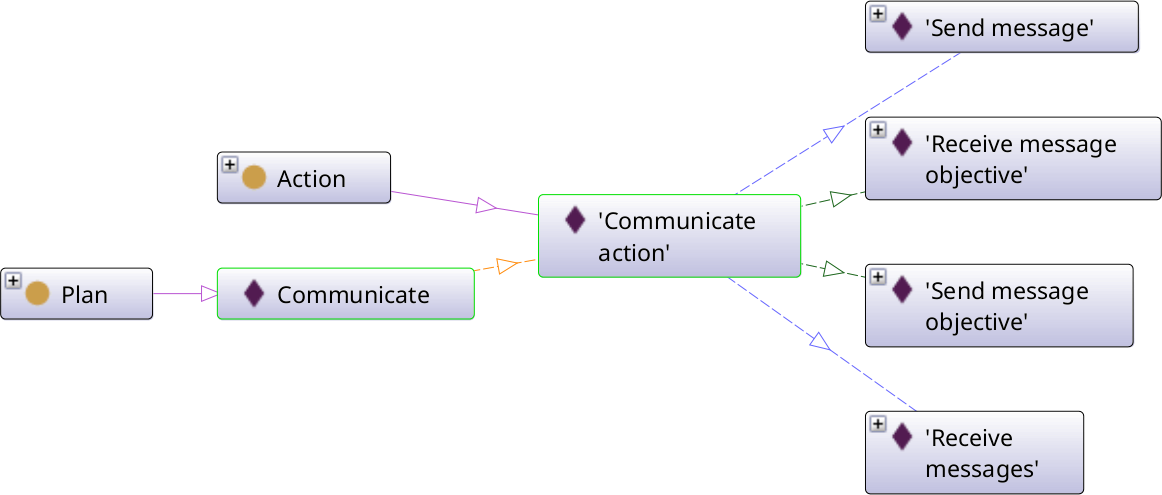
\includegraphics[width=\linewidth]{Deliverables/Phase 1/Figures/Example Communicate plan.png}
    \caption{Selected individuals related to the \mintedInline{Communicate} individual of concept \mintedInline{Plan}}
    \label{fig: Example Communicate plan}
\end{figure}

\begin{figure*}
    \centering
    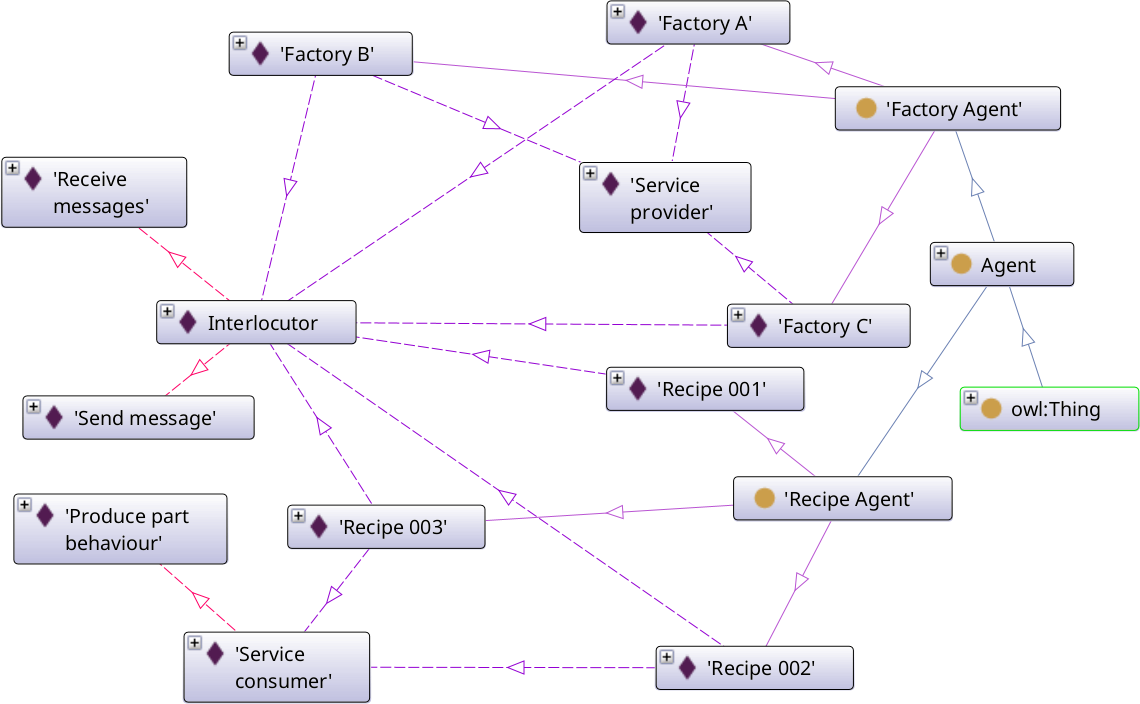
\includegraphics[width=\linewidth]{Deliverables/Phase 1/Figures/Example agents and roles.png}
    \caption{Agents of the example and their connected roles and behaviours they enable}
    \label{fig: Example agents and roles}
\end{figure*}

The modelled system is translated into the implementation template consisting of the following four files:
\begin{itemize}
    \item \mintedInline{Agent_Factory_Agent.py} is the place where the \mintedInline{Factory Agent} concept is translated into a \ac{SPADE} agent class.

    \item \mintedInline{Agent_Recipe_Agent.py} is the place where the \mintedInline{Recipe Agent} concept is translated into a \ac{SPADE} agent class.

    \item \mintedInline{Behaviours.py} is where all the \mintedInline{Behaviour} individuals' implementation templates are located.

    \item \mintedInline{Worksapce_workspace.py} contains agent instantiations and should be run if the modelled and now translated system is to be run.
\end{itemize}

% \begin{longlisting}
%     \mintedFilePython[]{Deliverables/Phase 1/Implementation/mago_thing.py}
%     \caption{The \mintedInline{mago_thing.py} file}
%     \label{lst: appendix mago-ag thing}
% \end{longlisting}

% \begin{longlisting}
%     \mintedFilePython[]{Deliverables/Phase 1/Implementation/mago_thing.py}
%     \caption{The \mintedInline{mago_thing.py} file}
%     \label{lst: appendix mago-ag thing}
% \end{longlisting}

% \begin{longlisting}
%     \mintedFilePython[]{Deliverables/Phase 1/Implementation/mago_thing.py}
%     \caption{The \mintedInline{mago_thing.py} file}
%     \label{lst: appendix mago-ag thing}
% \end{longlisting}

% \begin{longlisting}
%     \mintedFilePython[]{Deliverables/Phase 1/Implementation/mago_thing.py}
%     \caption{The \mintedInline{mago_thing.py} file}
%     \label{lst: appendix mago-ag thing}
% \end{longlisting}